% ITACA III working manuscript: adapted from notes/physics/nausica.tex.
% Springer Nature December 2024 template; EPJ C recommends iicol.
\documentclass[pdflatex,iicol,sn-mathphys-num]{sn-jnl}
\usepackage[T1]{fontenc}
\usepackage[utf8]{inputenc}
\usepackage{microtype}
\usepackage{amsmath,amssymb,graphicx,booktabs,array,mathtools}
\usepackage{xcolor,enumitem,tikz}
% Selected definitions imported from the ITACA manuscript on 2026-10-22.
% Source: /Users/jjgomezcadenas/Papers/itaca/pool/NextDefs.tex
% Used by itacaRevisited.tex alongside pool/NextLatexPackagesBase.tex.
% Local copy: compiling this note does not require the external directory.
% Preserve source macro names and notation; omit numerical design inputs,
% run-specific measurements, draft labels and conflicting SI unit aliases.
\usepackage{siunitx,xspace}
\sisetup{separate-uncertainty=true}

% Double-beta decay
\newcommand{\bb}{\ensuremath{\beta\beta}}
\newcommand{\bbonu}{\ensuremath{\beta\beta0\nu}}
\newcommand{\bbtnu}{\ensuremath{\beta\beta2\nu}}
\newcommand{\Qbb}{\ensuremath{Q_{\beta\beta}}}
\newcommand{\mbb}{\ensuremath{m_{\beta\beta}}}
\newcommand{\Tonu}{\ensuremath{T_{1/2}^{0\nu}}}
\newcommand{\Ttnu}{\ensuremath{T_{1/2}^{2\nu}}}
\newcommand{\Monu}{\ensuremath{\Big|M_{0\nu}\Big|}}
\newcommand{\Mtnu}{\ensuremath{\Big|M_{2\nu}\Big|}}
\newcommand{\Gonu}{\ensuremath{G_{0\nu}(\Qbb, Z)}}
\newcommand{\Gtnu}{\ensuremath{G_{2\nu}(\Qbb, Z)}}

% Isotopes and ion species
\newcommand{\XE}{\ensuremath{{}^{136}\rm Xe}}
\newcommand{\XEO}{\ensuremath{^{137}}Xe}
\newcommand{\BI}{\ensuremath{{}^{214}\rm Bi}}
\newcommand{\TL}{\ensuremath{{}^{208}\rm{Tl}}}
\newcommand{\KR}{\ensuremath{^{83m}\mathrm{Kr}}\xspace}
\newcommand{\Xe}[1]{\ensuremath{^{#1}\mathrm{Xe}}\xspace}
\newcommand{\Bi}[1]{\ensuremath{^{#1}\mathrm{Bi}}\xspace}
\newcommand{\Tl}[1]{\ensuremath{^{#1}\mathrm{Tl}}\xspace}
\newcommand{\Kr}[1]{\ensuremath{^{#1}\mathrm{Kr}}\xspace}
\newcommand{\xetp}{\ensuremath{{\rm Xe_2^{+}}}}
\newcommand{\batp}{\ensuremath{{\rm Ba^{2+}}}}
\newcommand{\nhfp}{\ensuremath{{\rm NH_4^{+}}}}
\newcommand{\nht}{\ensuremath{{\rm NH_3}}}

% Detector names and terminology
\newcommand{\NEW}{NEXT-White}
\newcommand{\NEXT}{NEXT-100}
\newcommand{\GXeEL}{GXeEL}
\newcommand{\HPXe}{HPXe}
\newcommand{\HPXeEL}{HPXe-EL}
\newcommand{\TM}{\emph{Topmetal}\xspace}

% Signals, transport and statistical notation
\newcommand{\tz}{\ensuremath{t_0}}
\newcommand{\sone}{\ensuremath{S_1}}
\newcommand{\stwo}{\ensuremath{S_2}}
\newcommand{\nph}{\ensuremath{n_\gamma}}
\newcommand{\VDR}{\ensuremath{v_d}}
\newcommand{\VD}{\ensuremath{v_d}}
\newcommand{\REF}{\ensuremath{\frac{E}{P}}}
\newcommand{\REY}{\ensuremath{\frac{Y}{P}}}
\newcommand{\chitwo}{\ensuremath{\chi^2}}
\newcommand{\SigmaE}{\ensuremath{\sigma_E / E}}
\newcommand{\stat}{\textrm{(stat.)}}
\newcommand{\sys}{\textrm{(sys.)}}

% Reference and table helpers
\newcommand{\fig}{figure}
\newcommand{\eq}{equation}
\newcommand{\tab}{table}
\newcommand{\Fig}{Figure}
\newcommand{\Eq}{Equation}
\newcommand{\Tab}{Table}
\newcommand{\minitab}[2][l]{\begin{tabular}{#1}#2\end{tabular}}

\graphicspath{{generated/}}
\setlength{\emergencystretch}{2em}
\setlist{nosep,leftmargin=*}
% Generated by scripts/benchmarks/build_physics.py; do not edit.
\newcommand{\OpenFraction}{0.04909}
\newcommand{\EntranceThreshold}{4.074}
\newcommand{\FluxRatio}{1.227}
\newcommand{\Mobility}{5}
\newcommand{\DiffusionCoefficient}{1.263}
\newcommand{\PeakCurrent}{1.731}
\newcommand{\DiskPeakCurrent}{1.923}
\newcommand{\FinalNinetyTime}{193.51}
\newcommand{\GapChargeFraction}{0.9984124}
\newcommand{\GapPotential}{0.0015876}
\newcommand{\GapMissingPercent}{0.1588}
\newcommand{\SquareHalfWidth}{0.25}
\newcommand{\GapSpeed}{3}
\newcommand{\ConfigHash}{628be0c9c8b9}

% Generated by scripts/benchmarks/build_readout.py; do not edit.
\newcommand{\SignalPadWidth}{0.5}
\newcommand{\SignalGap}{5}
\newcommand{\SignalGapField}{6}
\newcommand{\ReadoutCapacitance}{3}
\newcommand{\SingleIonIdealVoltage}{53.32}

% Generated from results/ltspice/discharge_calibration/20ms/paper_readout.h5; do not edit.
\newcommand{\SpicePadPf}{1.25}
\newcommand{\SpiceCfFf}{3}
\newcommand{\SpiceFrameMs}{20}
\newcommand{\SpiceAverageUs}{300}
\newcommand{\SpiceCorrectionSeconds}{2.454}
\newcommand{\SpiceTemperatureK}{293.15}
\newcommand{\SpiceLowHz}{0.1}
\newcommand{\SpiceHighMHz}{1}
\newcommand{\SpiceGainUv}{27.119}
\newcommand{\SpiceNoiseMv}{3.056}
\newcommand{\SpiceEncIons}{112.7}
\newcommand{\SpiceMinimumIons}{564}
\newcommand{\SpiceBelowIons}{563}
\newcommand{\SpiceBelowSnr}{4.9921}
\newcommand{\SpiceAboveSnr}{5.0009}
\newcommand{\SpicePreviousPercent}{0.082}
\newcommand{\SpiceFollowingPercent}{0.518}
\newcommand{\SpiceSupplyV}{1.8}

% Generated from results/ltspice/m3_scan/analysis.h5, scale_4_gate_0.5384774789.
\newcommand{\SpiceBaselineV}{0.879}
\newcommand{\SpicePowerUw}{344}

% Generated by figures/build_bias_values.py from paper_rounded_4.
\newcommand{\SpiceMthreeGateV}{0.5385}
\newcommand{\SpiceMfourGateV}{0.5568}
\newcommand{\SpiceBiasRoundingEncPercent}{0.06}
\newcommand{\SpiceBiasRoundingGainPercent}{0.27}

% Generated by figures/build_injection_values.py from the M3 x4 study.
\newcommand{\SpiceInjectionEnc}{55.4}
\newcommand{\SpiceInjectionCalibration}{100}

% Generated from results/ltspice/discharge_calibration/20ms/paper_readout.h5; do not edit.
\newcommand{\SpiceScanFirstEnc}{116.4}
\newcommand{\SpiceScanLastEnc}{111.7}

% Generated by figures/build_pixel_area.py
\newcommand{\PixelCellArea}{4}
\newcommand{\PixelBudgetArea}{1}
\newcommand{\PixelClearanceUm}{50}
\newcommand{\PixelDeviceMarginUm}{20}
\newcommand{\PixelOuterMarginUm}{40}
\newcommand{\PixelRowGapUm}{20}
\newcommand{\PixelCsaWidthUm}{200}
\newcommand{\PixelCsaHeightUm}{840}

\newcommand{\ion}{\ensuremath{\mathrm{Xe}_2^+}}
\newcommand{\dd}{\mathrm{d}}
\raggedbottom

\begin{document}
\title[NAUSICAA for ITACA]{NAUSICAA for ITACA}
\author[1]{\fnm{J. J.} \sur{G\'omez-Cadenas}}
\author[2]{\fnm{Vicente} \sur{Herrero}}
\author[3]{\fnm{Rogelio} \sur{Palomo}}
% Corresponding author and email to be supplied by the authors.
\affil[1]{\orgname{Donostia International Physics Center (DIPC)},
 \orgaddress{\street{Paseo Manuel de Lardizabal n\textsuperscript{o} 4},
 \city{Donostia-San Sebasti\'an}, \postcode{20018}, \state{Gipuzkoa}, \country{Spain}}}
\affil[2]{\orgname{Universidad Polit\'ecnica de Valencia}, \orgaddress{\country{Spain}}}
\affil[3]{\orgdiv{Dept. of Electronic Engineering, School of Engineering},
 \orgname{University of Sevilla}}
\abstract{ITACA (Ion Tracking Apparatus with CMOS ASICs) is a proposed new detector to search for neutrinoless double beta decay (\bbonu) events in a future, (multi) ton scale, ultra-low background, high pressure xenon TPC. The crucial innovation introduced by ITACA is the measurement of both the electron and the ion tracks produced in the xenon gas in response to ionizing particles. The readout of the ion track involves the use of electronics able to measure the charge carried by the positive xenon ions arriving at the cathode. We propose a design based on bare metal pads (TopMetal) coupled to CMOS electronics, which we call NAUSICA (Non-Amplified Ultra-Slow Ion CMOS ASIC). 

This paper presents a conceptual design of NAUSICA and a simplified model of its response to ion tracks. We use a Geant4-based simulation of ITACA to generate \bbonu\ events uniformly in the fiducial volume of the detector. The ions produced by each track drift to the cathode where they are focused towards the metal electrodes. We calculate the distribution of ion arrival positions and times after drift, diffusion and focusing and the current induced on each collection pad. A charge-sensitive amplifier (CSA) computes the voltage produced as this current is integrated on a feedback capacitor with a finite discharge time. We then add electronic noise and digitize the voltage to obtain the digitised signal from each pad. The combined response of all the pads with signals above a noise-dependent threshold allows the reconstruction of the track. We show that the track can be
resolved above the noise, keeping its characteristic topology.}
\maketitle


\section{Introduction}

The next generation of neutrinoless double-beta decay (\bbonu) experiments, aiming to establish if the neutrino is its own antiparticle, will attempt to explore very long lifetimes for a putative decay, $T_{1/2} > 10^{28}$~yr. This ambitious goal will require (multi) ton target masses of a suitable isotopes and detectors able to reduce backgrounds to a small fraction of one count per ton and year in the region of interest (ROI) near the end point of the decay (\Qbb) ~\cite{Gomez-Cadenas:2023vca}. 

High Pressure Xenon TPCs with electroluminescent readout (HPXeEL)~\cite{Gomez-Cadenas:2019ges} are one of the leading technologies for such a generation of large, virtually background-free \bbonu\ detectors. Their development has been pioneered by the NEXT collaboration, which is currently operating the NEXT-100 apparatus \cite{NEXT:2025yqw} at the Canfranc Underground Laboratory. NEXT-100 is the first realization of a large scale HPXeEL in the world. It holds $\sim100$~kg of xenon at 15~bar, in a TPC of roughly 1~m$^3$ volume.  
%NEXT has demonstrated a FWHM energy resolution of $(0.93 \pm 0.02)$\% at \Qbb~\cite{NEXT:2025ozn}. 

An HPXeEL provides two powerful handles to separate signal events from backgrounds. First, a very good energy resolution, measured by NEXT-100 to be $(0.93 \pm 0.02)$\% at \Qbb~\cite{NEXT:2025ozn}. Second, a distinctive topological signature that enables identification of events with two emitted electrons. A \bbonu\ candidate is defined as a single, continuous track, with no detached energy deposits and fully contained inside the fiducial volume. The energy of the track must be close to \Qbb\, typically within a ROI of $\pm 1$ FWHM.  This ``single-track'' requirement suppresses nearly all backgrounds, leaving only single-electron events with energies near \Qbb, such as those arising from photoelectric interactions (without an accompanying X-ray satellite) of the 2.448~MeV $\gamma$ ray of \BI\ and the 2.615~MeV $\gamma$ ray of \TL ---in those case where the second energy deposit is lost---, as well as from beta decays of $^{137}$Xe created by cosmogenic activation. In addition to the single track condition, requiring large local energy deposits (``blobs'') near the two endpoints of the track provides an additional suppression of single electron backgrounds that make it into the ROI. The effectiveness of this topological discrimination has been amply demonstrated by several NEXT studies~\cite{Ferrario:2015kta, Ferrario:2019kwg, NEXT:2021vzd, Kekic2021, NEXT:2021pjq}. 

However, the performance of the topological signature in an HPXeEL is limited by diffusion. As ionisation electrons drift through the dense gas, they undergo elastic scattering with the gas atoms, producing a charge cloud whose transverse size increases with the drift length. At long drifts, the transverse diffusion becomes very substantial (e.g, of the order of \SI{10}{mm} in pure Xenon). Using Xe-He mixtures (typically in proportion 0.85/0.15)  reduces it by a factor 2.5~\cite{Felkai:2017oeq, McDonald_2019, NEXT:2019oxh}.  

In two recent papers~\cite{Gomez-Cadenas:2025ect, itaca2026}, we proposed a new approach to improving the topological signature, that preserves EL amplification ---needed for energy resolution and a fast trigger--- while adding a second measurement of the event topology. Specifically, we proposed to record two complementary tracks for each event: the \emph{electron track}---the established signature in an HPXeEL TPC---and the \emph{ion track}, formed by the positive ions left along the original particle trajectory. The ion track exhibits diffusion at the millimeter level and its diffusion is anti-correlated with the electron track. Thus, the combination of both measurements provides a dramatic boost to topological discrimination.
The Ion Tracking Apparatus with CMOS ASICs (\textsc{ITACA})~\cite{itaca2026} is a proposed  HPXeEL based on this principle. The study presented there showed that reconstructing the ion track could increase the rejection power of the topological signature by more than one order of magnitude, leading to tiny background levels suitable for the exploration of \bbonu\ lifetimes in excess of $10^{28}$ years.

Reading the ions produced by a putative \bbonu\ event (or a single electron background in the ROI) is not easy, since, unless electrons, they cannot be amplified. In ~\cite{itaca2026}, we proposed an ion sensor based in the TopMetal concept~\cite{An2016TopmetalII, Gao2019TopmetalS, Yang2024TopmetalCSA, Liang2024TopmetalS}, which proposes to read the ions using bare metal pads (TopMetal) coupled to a Charge Sensitive Preamplifiers.

The idea of reading the (negative) ions left by ionizing tracks in a HPXe TPC was proposed in  ~\cite{Nygren_2018} in the context of a negative-ion TPC using ${}^82{\rm SeF_6}$ gas. It has been later adopted by the NvDev collaboration as the basics of their
proposal~\cite{NnDEx-100:2023alw}. In both cases, the experimental technique is based in reading exclusively the ion signal. 

Without entering in the feasibility of using SeF$_6$ due to experimental difficulties (the gas is toxic), a technique based on reading only the ions faces several problems. First, the tracks of the electrons propagating in the gas with energies closes to \Qbb~are long, of the order of 10-20 cm. Assuming drift velocities in the range $10--20$ cm/s, the typical time that takes to read the event is one second, resulting in potential pile-up from \bbtnu\ events~\cite{NnDEx-100:2023alw}. Second, the energy resolution needs to be measured from the ions themselves, which in turn implies an electronic noise very low and a modest number of pixels sharing the charge. Third, the track has to be reconstructed with sufficient detail by the electronics ---to match the excellent resolution afforded by the low diffusion--- which implies, on the contrary, a small pitch and therefore a large number of pixels. Thus, good energy resolution and a precise topology measurements impose contradictory requirements on the event reconstruction, and both demand an extraordinary performance of the electronics. 

The advantages of using an HPXeEL TPC with dual readout of the charge (electron and ions tracks) are: a) the event can be triggered with the fast electron track, which is readout in milliseconds, thus avoiding pileup; b) the energy is measured using proportional electroluminescence, with a proved resolution in the range of 0.7-0.9 \% FWHM at \Qbb; c) the ion readout can, therefore, be optimized for topology reconstruction. Furthermore, the fact that the EL measurement allows predicting both the time (to ms precision) and the point of arrival (to cm precision), allows the possibility of a movable ion detector, as discussed in ~\cite{itaca2026}. However, the requirement of extremely low noise electronics remains valid. 

%Reading the arriving ions (without amplification) requires exposed metal electrodes connected to charge-sensitive amplifiers (CSAs). Our proposed  \emph{Non-Amplified Ultra-Slow Ion CMOS ASIC} (NAUSICA) uses TopMetal CMOS technology~\cite{An2016TopmetalII} to implement this concept, following Refs.~\cite{Nygren_2018, mei2020topmetalcmosdirectcharge}. There is an important difference, however, with respect to these works, which attempted to design a system able to provide simultaneously good energy resolution and a good measurement of the track topology using ions. Alas, both requirements impose constraints that interfere with each other. Good energy resolution requires optimizing ion counting and minimizing noise. Good topological reconstruction demands pixels separated by a small pitch (e.g., of the order of diffusion, $\sim 2$ mm), which in turn multiplies the number of pixels and adds to the overall noise. The advantage of ITACA is that energy resolution is measured with excellent precision by electroluminescence, and thus the ion detector can prioritize the reconstruction of the topology. NAUSICA is designed with this goal in mind. Appendix~\ref{app:topmetal} compares its geometry and charge-injection noise with Topmetal-S.


In this paper we present a conceptual design of NAUSICA (Non-Amplified Ultra-Slow Ion CMOS ASIC), our proposed readout for ITACA and offer a full quantification of its performance. 
%Our study~\cite{itaca2026} Here we show that the proposed NAUSICA readout can preserve the resolution at the level dictated by the diffusion, thus guaranteeing the expected enhancement of the topology discrimination power.
%
The organization is as follows. Section \ref{sec:itaca_det} briefly summarizes the main aspects of the ITACA detector. 
Section \ref{sec:nausica} presents the NAUSICA concept.
% TODO: Complete the roadmap after the new sections are in place.


\section{The ITACA Detector}
\label{sec:itaca_det}


%The pressure of operation in ITACA is chosen as a tradeoff between mass --- which increases with pressure --- and track topology, which is easier to resolve at lower pressure. Other considerations include ion drift velocity, which decreases approximately inversely with pressure at fixed electric field, and electron lifetime, which tends to improve at lower pressure. Overall, 15 bar is a good compromise. Using electroluminescence to amplify the electron track signal guarantees excellent energy resolution. Fiducialisation of the event requires the measurement of $t_0$, provided by primary scintillation. Both requirements are essential for a \bbonu\ experiment.
 
 \begin{figure*}[!htbp]
    \centering
    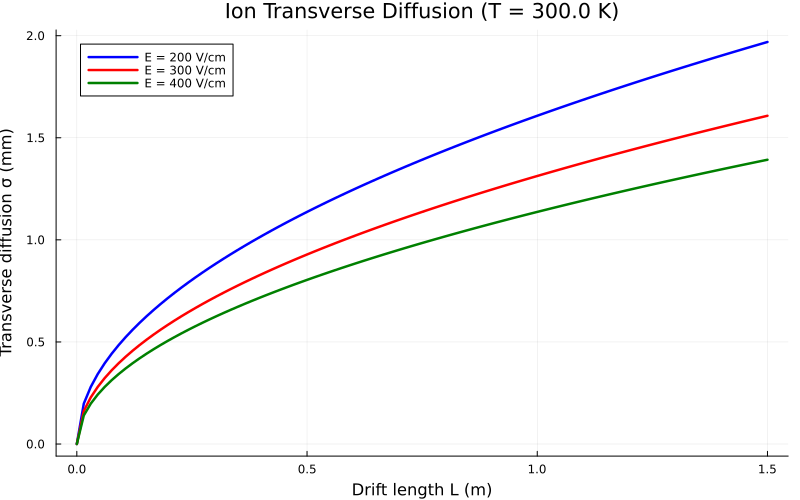
\includegraphics[width=0.48\textwidth]{img/ion_diffusion_vs_length.png}
     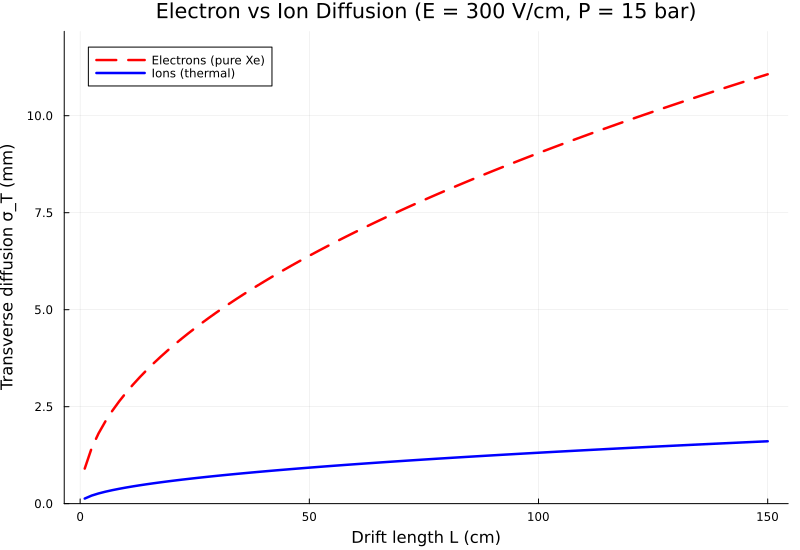
\includegraphics[width=0.48\textwidth]{img/electron_ion_diffusion.png}
    \caption{Left: transverse diffusion of \xetp\ ions as a function of drift length for three different drift fields; right: transverse diffusion of \xetp\ ions compared with transverse diffusion of electrons in pure xenon.}
    \label{fig:sigmatvsl}
\end{figure*}
 
 
\begin{table}[htbp]
\centering
\caption{Summary of ITACA detector parameters.}
\label{tab:itaca_params}
\begin{tabular}{@{}llrl@{}}
\toprule
\textbf{Parameter} & \textbf{Symbol} & \textbf{Value} & \textbf{Unit} \\
\midrule
\multicolumn{4}{@{}l}{\textit{Geometry}} \\
Fiducial diameter      & $D_{\mathrm{fid}}$   & 320   & cm \\
Fiducial height        & $L_{\mathrm{fid}}$   & 150   & cm \\
Fiducial volume        & $V_{\mathrm{fid}}$   & 12.1  & m$^3$ \\
Fiducial Xe mass       &                      & 1050  & kg \\
PV internal diameter   &                      & 3.54  & m \\
PV internal height     &                      & 2.01  & m \\
\midrule
\multicolumn{4}{@{}l}{\textit{Electric field and drift}} \\
Drift field            & $E$                  & 200   & V/cm \\
Electron drift velocity& $v_e$                & 1     & mm/$\mu$s \\
Electron drift time    & $t_e$                & 1.5   & ms \\
Ion drift velocity     & $v_d$                & 10    & cm/s \\
Ion drift time (max)   & $t_{\mathrm{max}}$   & 15    & s \\
\bottomrule
\end{tabular}
\end{table}

ITACA is a proposed HPXeEL TPC implementing the readout of both the ion and the electron track. Its dimensions and operation pressure are chosen to accommodate 1 ton of gas in the fiducial region, and are described in 
~\cite{itaca2026} and summarized in Table~ \ref{tab:itaca_params}.
 %Choosing the detector dimensions implies a tradeoff between the diameter and the length of the TPC. 
 A major design goal is to minimise the transverse diffusion $\sigma_T$ of ions, which in the thermal limit is simply:
 %
 \begin{equation}
\sigma_T =\sqrt{\tfrac{2k_BT}{q_e}\tfrac{L}{E}} 
\label{eq:drift}
\end{equation}
%
where $L$ is the ion drift distance, $E$ the drift field, $T$ the gas temperature, $k_B$ Boltzmann's constant and $q_e$ the elementary charge. Equation~\ref{eq:drift} favours shorter $L$ and larger $E$. Figure~\ref{fig:sigmatvsl} shows $\sigma_T$ for three different drift fields. For a TPC drift length of 150~cm, the average $\sigma_T$ is of the order of \SI{1}{mm}, one order of magnitude smaller than the corresponding diffusion for electrons in pure xenon. Once the length of the TPC is defined, the diameter of the TPC defines the fiducial mass that can be achieved. At 15 bar, choosing $D= 320$ cm, results in a fiducial mass slightly above one ton, $M_{fid} = 1050$ kg. 
 
A large diameter TPC requires modular instrumentation of both the EL side (with pixels sensitive to light) and the cathode side (with pixels sensitive to bare ion charge). There is no charge amplification in the cathode, but an intense field

In addition, one has to provide a system to measure the energy of the event with excellent resolution. ITACA is equipped with a Barrel Fibre Detector (BFD) able to measure both primary scintillation (\sone) and secondary, EL scintillation (\stwo). The measurement of \sone\ provides the start-of-the-event, \tz\, needed to fiducialize it. The measurement of \stwo\ provides a measurement of the energy, to a resolution 
of the order of 0.7\% FWHM at \Qbb. 

The anode is equipped with a HELM device, whose role is to provide the EL light needed for the BFD and a measurement of the electron track topology. 

%The cathode side

%Another important design factor is the voltages in the TPC electrodes. All sensors (the CMOS reading the ions and the SiPMs reading the EL light) operate best at ground, but the drifting of electrons and ions requires a constant field in the TPC, and the generation of EL light requires an additional, higher field, in the EL region. 

The cathode is instrumented with an Ion Focusing Grid (IFG) which focuses the incoming ions into the readout pads of the CMOS detector. The upper electrode of the IFG is at a voltage $V_c = \SI{8}{kV}$. The voltage on the anode side of the TPC depends on the drift length and the drift field. A good compromise between minimizing diffusion and keeping voltage at the anode reasonable is to choose a drift field of \SI{200}{V/cm}, which results in \SI{38}{kV} at the first anode electrode, and \SI{54}{kV} at the second (with \SI{16}{kV} across the EL gap). 
 
 
 A large diameter TPC requires instrumenting both the EL side (with SiPMs) and the cathode side (with top metal devices). 
  Previous work involving the detection of
 ions for \bbonu\ experiments \cite{Nygren_2018, mei2020topmetalcmosdirectcharge} has quantified the challenge of instrumenting a large surface with CMOS detectors, which appears, nonetheless, feasible \cite{You2021}. The ITACA paper~\cite{itaca2026} proposes a movable ion detector, the Magnetically Actuated Rotor System (MARS). The NAUSICA readout considered here could be used as part of MARS or to instrument the full cathode.  Table~\ref{tab:itaca_params} shows the main parameters of a 1-ton ITACA detector. 

% =================================================================
\subsection{Principle of operation}
\label{sec:pof}

Consider a putative \bbonu\ event occurring in the middle of the TPC. Two electrons, with a total energy of \Qbb\ (\SI{2458}{keV}), propagate through the dense noble gas, ionising it. Primary scintillation is recorded and a fast trigger system (FTS) records the start-of-the-event $t_0$. Then a fast measurement of the event energy is performed, accepting the event only if its energy lies within a pre-determined ROI (selected to be $\pm 1\sigma$ around \Qbb). Events outside the ROI are rejected and no ion readout is attempted.

Since the event that we are considering is a \bbonu\ decay, the FTS will likely trigger, activating a fast reconstruction of the topology and event barycenter, $(x_i, y_i, z_i)$. The coordinates $(x_i,y_i)$ predict the landing position of the ion cloud at the cathode, while $z_i$, together with $t_0$ and the ion drift velocity, determines the arrival time of its barycenter ($t_i$). 

     
The \xetp\ ions reach the cathode on a time scale of seconds. In our specific example, with the event at the midpoint of the TPC, they need to drift \SI{75}{cm} at a velocity of \SI{10}{cm/s}, requiring \SI{7.5}{s}. 
The typical longitudinal extension of the ion track is of the order of \SI{10}{cm}, and thus about \SI{1}{s} is needed to collect the ions. 

Notice that the electron track and the ion track are detected in \emph{delayed coincidence}. The ion track is intercepted precisely at the right time and in the right place, thus minimising the impact of spurious coincidences. At the expected trigger rate (dominated by backgrounds in the ROI), pile-up during the $\sim$\SI{15}{s} maximum ion drift time is negligible.


\section{The NAUSICA concept}
\label{sec:nausica}

Reading the arriving ions (without amplification) requires exposed metal electrodes connected to charge-sensitive amplifiers (CSAs). Our proposed  \emph{Non-Amplified Ultra-Slow Ion CMOS ASIC} (NAUSICA) uses TopMetal CMOS technology~\cite{An2016TopmetalII} to implement this concept, following Refs.~\cite{Nygren_2018, mei2020topmetalcmosdirectcharge}. There is an important difference, however, with respect to these works, which attempted to design a system able to provide simultaneously good energy resolution and a good measurement of the track topology using ions. Alas, both requirements impose constraints that interfere with each other. Good energy resolution requires optimizing ion counting and minimizing noise. Good topological reconstruction demands pixels separated by a small pitch (e.g., of the order of diffusion, $\sim 2$ mm), which in turn multiplies the number of pixels and adds to the overall noise. The advantage of ITACA is that energy resolution is measured with excellent precision by electroluminescence, and thus the ion detector can prioritize the reconstruction of the topology. NAUSICA is designed with this goal in mind. Appendix~\ref{app:topmetal} compares its geometry and charge-injection noise with Topmetal-S.

Consider the \bbonu\ event that we described in the previous section. Assume the extreme case in which the track extends along $z$. For a track length of 10 cm and a drift velocity of 10 cm/s it would take one second, since the arrival of the first ions, to collect the full track. In practice, the tracks are oriented in random directions, extending radially over several pads, and collection of ions is faster, since few tracks extend exactly along $z$. In any case,  the resolution in $z$ is of the order of the transverse diffusion, ($\sigma_z = 1-2$ mm), so reading the charge in frames of 10-20 ms is reasonable. We take \SI{\SpiceFrameMs}{ms} as the nominal frame duration, corresponding to \SI{2}{mm} along the drift direction.
%The mean number of ions per pad in those buckets helps determine the feedback capacitance of the CSA.


\begin{figure*}[tbp]
    \centering
    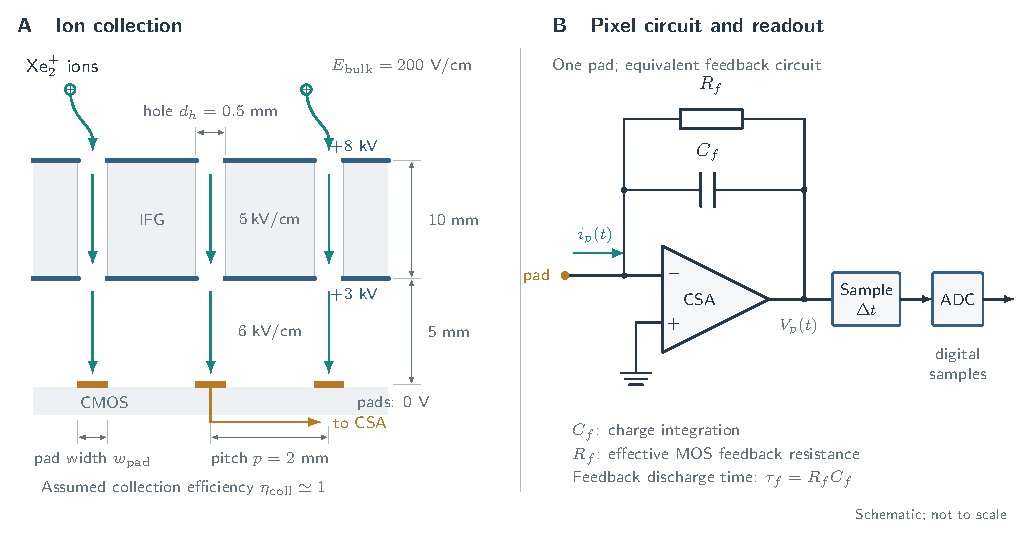
\includegraphics[width=\linewidth]{figures/nausica_concept.pdf}
    \caption{NAUSICA ion collection geometry (left) and equivalent pixel circuit (right). The drawing is schematic and not to scale.}
    \label{fig:nausicaa}
\end{figure*}


\subsection{Charge collection and focusing}

The pad dimensions and pitch need to be chosen balancing the desired spatial resolution with the need for an acceptable signal-to-noise (S/N) per pad. Larger pads increase the collection but also the input capacitance, thus the need to focus the incoming ions in an area as small as possible. The left panel of Fig. \ref{fig:nausicaa} shows a schematic of the Ion Focusing Grid (IFG), which does this job.  We estimate the focusing requirement by comparing the electric flux through one pixel cell with that through its hole. Taking uniform fields in the drift region and inside the hole, full flux collection requires
\[
E_h\,\frac{\pi d_h^2}{4}\gtrsim E_{\rm bulk}p^2.
\]
Here $E_h$ and $E_{\rm bulk}$ are the fields inside the hole and in the drift region, respectively, $d_h$ is the hole diameter, and $p$ is the pixel pitch.
For a pitch of 2 mm, a bulk field of 200 V/cm and a hole field of 5 kV/cm, this gives a minimum hole diameter of approximately 0.45 mm. Thus, we take 0.5 mm as a preliminary design parameter. We use square pads of 0.5 mm side on a 2 mm pitch. Full flux collection in this simple geometry implies a large ion collection efficiency that we take as one for the time being.


\subsection{Pixel electronics and readout}

The right panel of Fig. \ref{fig:nausicaa} shows a schematic of the electronics. Each pad is directly connected to the input of a CSA. The input current is integrated on a feedback capacitor $C_f$. A MOS transistor allows $C_f$ to discharge slowly. For an ideal CSA, the gain is $1/C_f$ and the signal decays with time constant $\tau_f$.


The sampled voltage includes charge accumulated in previous buckets. The charge arriving in each bucket is recovered from the change between successive samples, accounting for feedback discharge. We use frames of \SI{\SpiceFrameMs}{ms}. Each voltage reading is averaged over \SI{\SpiceAverageUs}{\micro\second}, as described in Section~\ref{sec:frame_readout}. This requires repeated digitisation within the acquisition window or an averaging stage before the ADC.

Digitisation could use ADCs shared by groups of pixels and mounted on readout boards behind the collection plane. Buffered pixel outputs would be multiplexed to these ADCs, with sufficient sampling to perform the averaging described above.

\subsection{Parameters of the design}

In summary, the pad size, pitch and active area must be chosen to sample and contain the ion track. The feedback capacitance and discharge time depend on the charge arriving at each pad and its distribution in time. The sampling interval, electronic noise and ADC range must allow the weaker parts of the track to be recorded while accommodating the largest signals.


\section{Signal formation and response of one pad}
\label{sec:single_ion}

Consider an ion, with charge $q=e$, arriving at a readout pad. The process of signal formation can be viewed in two steps:
\begin{enumerate}
\item As the ion approaches, a current is induced in the pad. 
\item Then the CSA integrates it and produces the voltage sampled by the readout.
\end{enumerate}

Next, we describe each step:

\subsection{The induced current}

The weighting potential of a pad, $\phi_{w}(r)$, describes how an ion’s motion contributes to the signal on that pad. We calculate it for the detector geometry with the following boundary conditions: (a) the selected pad is held at unit potential and (b) all other electrodes at zero. Also the calculation is performed in the absence of charge. 

We define positive current as current delivered into the CSA input by an approaching positive ion. With this convention, the meaning of $\phi_w$ follows from the Shockley--Ramo relation~\cite{riegler2016}
\begin{equation}
 \Delta Q=e\,\Delta\phi_w.
 \label{eq:single_charge}
\end{equation}

The current is the rate at which this signal develops:
\begin{equation}
 i_1(t)=e\frac{\dd\phi_w(\mathbf r(t))}{\dd t}.
 \label{eq:single_ramo}
\end{equation}
Near a small pad, $\phi_w$ changes rapidly with position, so most of the signal is induced during the final approach. 

For the analytical calculation we use a square pad of side $2a$, embedded in an infinite grounded plane. The gas occupies a homogeneous half-space above the plane. The ion approaches the centre of the pad along its normal at constant speed $v$. The gap width $g$ is the distance between the lower IFG electrode and the pad plane. This geometry provides a simple pad response. In this simple approximation, the IFG and the dielectric structure of the CMOS surface are not included in its weighting potential. Figure~\ref{fig:weighting_boundary} illustrates the geometry and weighting-potential boundary conditions. Appendix~\ref{app:single_ion} gives the derivation.

\begin{figure}[!htbp]
 \centering
 \resizebox{0.94\linewidth}{!}{% Square-pad weighting boundary conditions; included by nausica.tex.
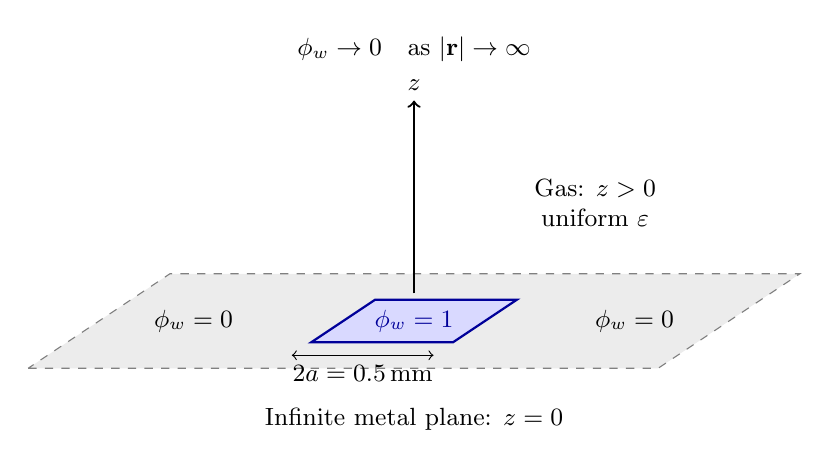
\begin{tikzpicture}[x={(1cm,0cm)},y={(0.45cm,0.3cm)},z={(0cm,1cm)},
                    font=\small]
 \fill[gray!15] (-4,-2,0) -- (4,-2,0) -- (4,2,0) -- (-4,2,0) -- cycle;
 \draw[dashed,gray] (-4,-2,0) -- (4,-2,0) -- (4,2,0) -- (-4,2,0) -- cycle;
 \filldraw[fill=blue!15,draw=blue!60!black,thick]
   (-0.9,-0.9,0) -- (0.9,-0.9,0) -- (0.9,0.9,0) -- (-0.9,0.9,0) -- cycle;
 \node[blue!60!black] at (0,0,0) {$\phi_w=1$};
 \node at (-2.8,0,0) {$\phi_w=0$};
 \node at (2.8,0,0) {$\phi_w=0$};
 \draw[->,thick] (0,0,0.35) -- (0,0,2.8) node[above] {$z$};
 \node[align=center] at (2.3,0,1.5) {Gas: $z>0$\\uniform $\varepsilon$};
 \node at (0,0,3.45)
   {$\phi_w\to0\quad\text{as }|\mathbf r|\to\infty$};
 \draw[<->] (-0.9,-1.45,0) -- (0.9,-1.45,0)
   node[midway,below] {$2a=\SI{\SignalPadWidth}{mm}$};
 \node at (0,0,-1.25) {Infinite metal plane: $z=0$};
\end{tikzpicture}
}
 \caption{Boundary conditions for the square-pad weighting potential.
 The drawing shows a portion of the infinite metal plane; the dashed outline
 indicates its continuation. The pad has $\phi_w=1$ and the surrounding metal
 $\phi_w=0$. In the gas, the potential satisfies Laplace's equation and tends
 to zero at infinity. Schematic, not to scale.}
 \label{fig:weighting_boundary}
\end{figure}

Place the pad at $z=0$ and take collection to occur at $t=0$, so that $z=-vt$ before collection. The weighting field on the central axis is
%
\begin{equation}
 W(z)=-\frac{\dd\phi_w}{\dd z}
 =\frac{4a^2}{\pi(z^2+a^2)\sqrt{z^2+2a^2}}.
 \label{eq:single_weight}
\end{equation}
%
For an ion entering this gap at $z=g$ and $t_g=-g/v$, the current is
%
\begin{equation}
 i_1(t)=
 \begin{cases}
 evW(-vt),&t_g\leq t<0,\\
 0,&\text{otherwise}.
 \end{cases}
 \label{eq:single_current}
\end{equation}
%
Its integral over this finite trajectory is $Q_g=e[1-\phi_w(g)]$.

\subsection{Signal size and duration}

As a numerical example, we take the parameters shown in the left panel of Fig. \ref{fig:nausicaa}: a pad of side \SI{\SignalPadWidth}{mm} and a gap of \SI{\SignalGap}{mm}. We estimate the gap velocity from $v=\mu E_g$, using the mobility inferred from the bulk drift speed and assuming it remains constant in the gap. With $E_g=\SI{\SignalGapField}{kV/cm}$, this gives $v=\SI{\GapSpeed}{m/s}$. 

The current rises as the ion approaches the pad and reaches
\begin{equation}
 i_1(0^-)=\frac{2\sqrt{2}}{\pi}\frac{ev}{a}
 =\SI{\PeakCurrent}{fA}.
 \label{eq:single_peak}
\end{equation}
%
Most of the signal is induced close to the pad (Figure~\ref{fig:single_ion_current}). The final $\sim$\SI{200}{\micro\second} before collection contain 90\% of the full-path charge $e$ \footnote{Here ``full path'' means extending the same analytical trajectory to infinite distance.}. For the finite gap used in the calculation (Appendix~\ref{app:single_duration}),
%
\begin{equation}
 Q_g=e[1-\phi_w(g)]=\GapChargeFraction\,e.
 \label{eq:single_gap_charge}
\end{equation}
%

\begin{figure*}[tbp]
 \centering
 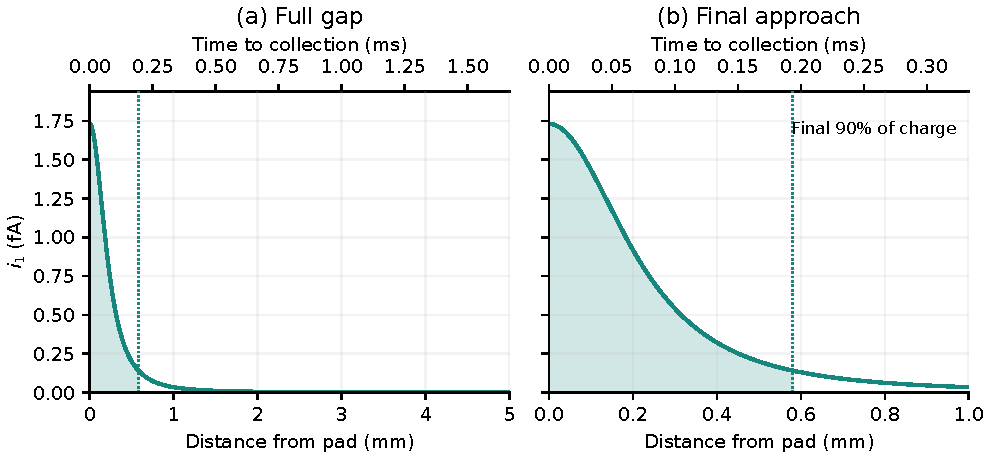
\includegraphics[width=\linewidth]{single_ion_current.pdf}
 \caption{Single-ion current across the full gap (left) and during the final approach (right), for the square-pad model described above. The upper axes show the time remaining before collection. The shaded region contributes 90\% of the full-path charge.}
 \label{fig:single_ion_current}
\end{figure*}

\subsection{Ideal CSA response}
\label{sec:ideal_csa}

%Consider an ion approaching the pad and reaching it at $t=0$.

We first describe the CSA by an ideal amplifier with feedback capacitance $C_f$ and an effective linear resistance $R_f$ representing the MOS discharge path. Consider an ion approaching the pad and reaching it at $t=0$.  The ion induces an input current $i_1(t)$, shared between the feedback capacitor and the discharge path. The resulting output voltage $V_1$, measured relative to its baseline, satisfies:
\begin{equation}
 i_1(t)=-C_f\frac{\dd V_1}{\dd t}-\frac{V_1}{R_f}.
 \label{eq:csa_current_balance}
\end{equation}
The first term describes charge integration and the second feedback discharge. With the discharge time $\tau_f=R_fC_f$, this becomes
%
\begin{equation}
 \frac{\dd V_1}{\dd t}+\frac{V_1}{\tau_f}
 =-\frac{i_1(t)}{C_f}.
 \label{eq:csa_ode}
\end{equation}
%
We assume that no signal is stored in the CSA when the ion enters the gap at $t=t_g$. Since $V_1$ is measured relative to the baseline, $V_1(t_g)=0$, and the solution is
\begin{equation}
 V_1(t)=-\frac{1}{C_f}\int_{t_g}^{t}
 i_1(t')\exp\left[-\frac{t-t'}{\tau_f}\right]\dd t'.
 \label{eq:csa_solution}
\end{equation}
With this convention positive input current produces a negative voltage. Once collection is complete, the voltage decays exponentially, $V_1(t)=V_1(0)\exp(-t/\tau_f)$.

Neglecting feedback discharge during the approach of one ion, the integral
at collection, $t=0$, gives
\[
 V_1(0)=-\frac{1}{C_f}\int_{t_g}^{0}i_1(t')\,\dd t'
 =-\frac{Q_g}{C_f}.
\]
For $C_f=\SI{\SpiceCfFf}{fF}$, its magnitude is
\SI{\SingleIonIdealVoltage}{\micro\volt}.

For several ions following the same final trajectory and collected on the
same pad at times $t_k$, the currents and voltages add:
\begin{equation}
 i_p(t)=\sum_k i_1(t-t_k),\qquad
 V_p(t)=\sum_k V_1(t-t_k).
 \label{eq:pad_superposition}
\end{equation}
The voltage therefore includes contributions from earlier arrivals that
have not yet discharged.

% Previous ideal-response plots and finite-gain section are preserved in
% archive/2026-10-26_pre_spice/reviewed_sections.tex.

\section{CSA response and noise}
\label{sec:realistic_csa}

A real amplifier has finite gain and bandwidth. The output voltage for a given
charge is smaller than the ideal value $Q/C_f$, and takes time to develop.
Electronic noise also sets a limit on the minimum charge that can be measured.
We calculate these effects using a transistor circuit in SPICE, with the
ion-induced current from Section~\ref{sec:single_ion} as its input.

\subsection{Circuit and operating parameters}
\label{sec:spice_circuit}

Figure~\ref{fig:spice_circuit} shows the CSA used in the calculation. It has a
PMOS input transistor, a folded-cascode amplifier and a feedback capacitor
$C_f$. An NMOS transistor, $M_f$, provides the discharge path. The circuit
uses 180 nm CMOS device models and a supply of \SI{\SpiceSupplyV}{V}.
The transistor dimensions are given in Table~\ref{tab:spice_devices}.
The DC operating-point calculation gives an output voltage of
\SI{\SpiceBaselineV}{V} and a quiescent power consumption of
\SI{\SpicePowerUw}{\micro\watt} for the CSA.

% Previous circuit drawing retained for review.
% \begin{figure}[!htbp]
%  \centering
%  \includegraphics[width=0.85\linewidth]{spice_circuit.pdf}
%  \caption{CSA circuit used in the SPICE calculation. Gate bias voltages and
%  drain (D) and source (S) connections are shown. The pad current enters the
%  gate of M1; $C_f$ and $M_f$ connect the output to this input node.}
%  \label{fig:spice_circuit}
% \end{figure}

\begin{figure}[!htbp]
 \centering
 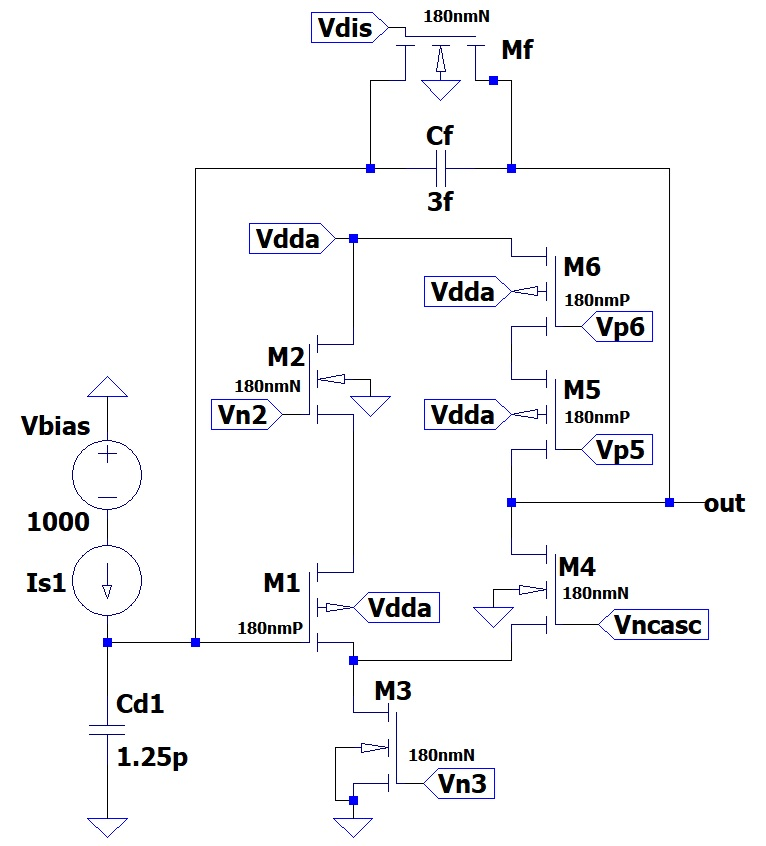
\includegraphics[width=0.78\linewidth,height=0.65\textheight,keepaspectratio]{figures/Nausica_Image.jpg}
 \caption{CSA circuit used in the SPICE calculation. The pad current enters
 the gate of M1; $C_f$ and $M_f$ connect the output to this input node.
 Transistor dimensions and operating parameters are given in
 Tables~\ref{tab:spice_devices} and~\ref{tab:spice_parameters}.}
 \label{fig:spice_circuit}
\end{figure}

\begin{table}[!htbp]
 \centering
 % Generated from LTSpice/variants/m4_x4_m3_x4/uniform_1000_ions.cir.
\begin{tabular}{llrrr}
\toprule
Device & Type & $W$ ($\mu$m) & $L$ ($\mu$m) & $m$ \\
\midrule
M1 & PMOS & 220 & 0.5 & 1 \\
M2 & NMOS & 27 & 0.5 & 3 \\
M3 & NMOS & 200 & 2 & 1 \\
M4 & NMOS & 2.88 & 1.44 & 1 \\
M5 & PMOS & 220 & 0.5 & 1 \\
M6 & PMOS & 1 & 6 & 1 \\
$M_f$ & NMOS & 0.36 & 100 & 1 \\
\bottomrule
\end{tabular}

 \caption{Transistor dimensions used in the SPICE calculation.}
 \label{tab:spice_devices}
\end{table}

The pad capacitance $C_{\rm pad}=\SI{\SpicePadPf}{pF}$ for
our \SI{\SignalPadWidth}{mm} pads is estimated from conservative scaling
of the Topmetal-S capacitance~\cite{Gao2019TopmetalS}.
%The device models include the transistor capacitances in addition to
%$C_{\rm pad}$. 
Table~\ref{tab:spice_parameters} lists the circuit and
readout parameters used below.

\begin{table}[!htbp]
 \centering
 \begin{tabular}{llr}
 \toprule
 Parameter & Symbol & Value \\
 \midrule
 External pad capacitance & $C_{\rm pad}$ & \SI{\SpicePadPf}{pF} \\
 Feedback capacitance & $C_f$ & \SI{\SpiceCfFf}{fF} \\
 Supply voltage & $V_{DD}$ & \SI{\SpiceSupplyV}{V} \\
 M3 gate voltage & $V_{\rm nload}$ & \SI{\SpiceMthreeGateV}{V} \\
 M4 gate voltage & $V_{\rm ncasc}$ & \SI{\SpiceMfourGateV}{V} \\
 Temperature & $T$ & \SI{\SpiceTemperatureK}{K} \\
 \midrule
 Frame duration & $\Delta t$ & \SI{\SpiceFrameMs}{ms} \\
 Averaging time & $T_a$ & \SI{\SpiceAverageUs}{\micro\second} \\
 Discharge-correction time & $\tau_0$ & \SI{\SpiceCorrectionSeconds}{s} \\
 Noise integration band & $[f_\ell,f_h]$ &
 \SI{\SpiceLowHz}{Hz}--\SI{\SpiceHighMHz}{MHz} \\
 \bottomrule
 \end{tabular}
 \caption{Parameters of the circuit and frame measurement. Gate bias voltages
 are rounded to four decimal places. The time $\tau_0$
 is obtained from the simulated voltage decay and used in the correction
 between readings.}
 \label{tab:spice_parameters}
\end{table}

\subsection{Response to uniform arrivals}
\label{sec:arrival_cases}

We consider $N$ ions arriving uniformly over a frame of duration $\Delta t$.
The number of ions is left to be determined from the required S/N.
Averaging the single-ion current over the collection time $u$ gives
\begin{equation}
 i_N(t)=\frac{N}{\Delta t}\int_0^{\Delta t}i_1(t-u)\,\dd u.
 \label{eq:uniform_arrival_current}
\end{equation}
The currents overlap, producing an approximately constant current through
most of the frame. The voltage builds up during this interval.
The current is supplied to SPICE as a table of times and values, with its
integral fixed by the finite-gap charge $NQ_g$.

\begin{figure}[!htbp]
 \centering
 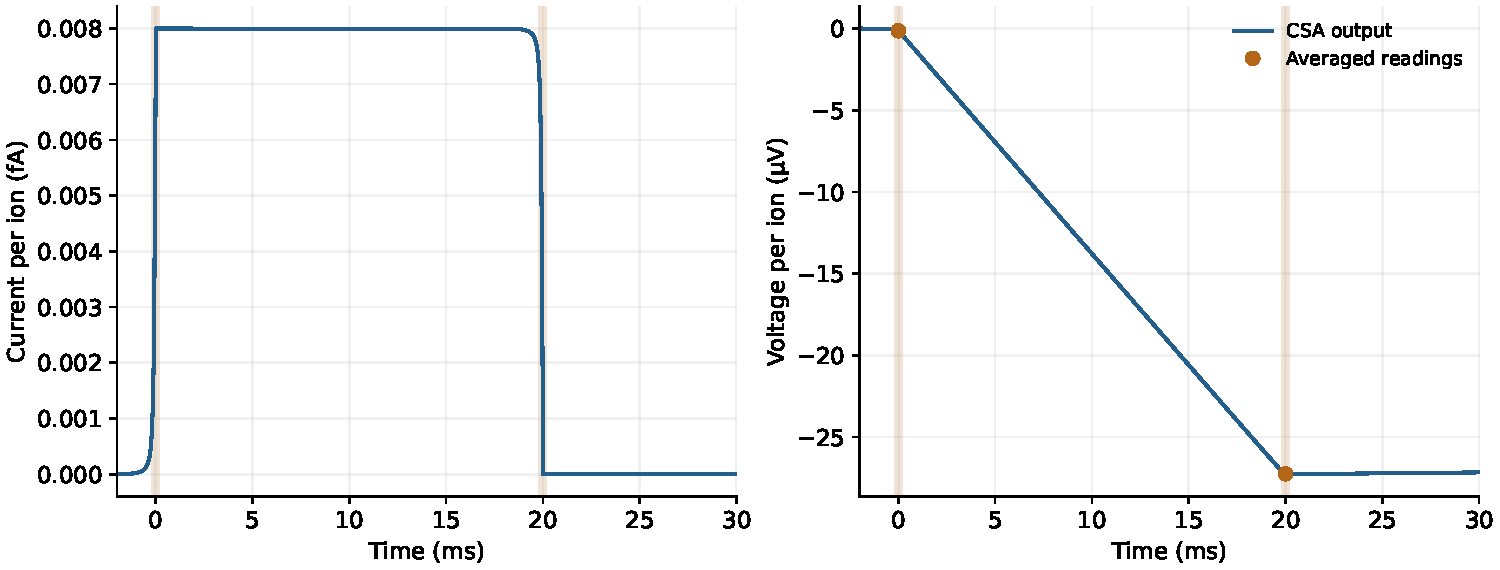
\includegraphics[width=\linewidth]{spice_ion_response.pdf}
 \caption{Uniform ion arrivals over a \SI{\SpiceFrameMs}{ms} frame.
 Left: input current per ion. Right: SPICE output voltage relative to the
 baseline, per ion. The shaded windows have width
 \SI{\SpiceAverageUs}{\micro\second}; the points show the averaged voltages.}
 \label{fig:spice_ion_response}
\end{figure}

Figure~\ref{fig:spice_ion_response} shows the current and voltage normalized
to one ion. Since the voltage remains after the arrival interval, successive
frames must be treated as a continuous signal.

\subsection{Frame readout}
\label{sec:frame_readout}

The voltage at each frame boundary is averaged over a window of duration $T_a=\SI{\SpiceAverageUs}{\micro\second}$, large enough to average the rapid voltage fluctuations that would enter a point
reading, but much shorter than
the \SI{\SpiceFrameMs}{ms} frame.
\begin{equation}
 \overline V_n=\frac{1}{T_a}
 \int_{t_n-T_a/2}^{t_n+T_a/2}V(t)\,\dd t,
 \qquad t_n-t_{n-1}=\Delta t.
 \label{eq:spice_average}
\end{equation}

When discussing the ideal CSA, we saw that the residual voltage decays exponentially, 
$\exp(-\Delta t/\tau_f)$. This motivates the corrected voltage difference
\begin{equation}
 D_n=-\left(\overline V_n-\alpha\overline V_{n-1}\right),
 \qquad \alpha=\exp(-\Delta t/\tau_0).
 \label{eq:spice_frame_difference}
\end{equation}
which takes into account  the voltage left from the previous frame. 
The minus sign makes $D_n$ positive for the chosen output polarity.
We determine the value of $\tau_0$ ($\tau_0=\SI{\SpiceCorrectionSeconds}{s}$) by fitting an exponential to the SPICE output voltage,
measured relative to its baseline, after the ion current has ended. We then calibrate the resulting
measurement with the SPICE response. Let $g$ be
$D_n$ for the uniform current normalized to one ion. In the linear regime,
$N$ ions give $Ng$, and their estimated number is
\begin{equation}
 \widehat N_n=\frac{D_n}{g}.
 \label{eq:spice_calibration}
\end{equation}
Applying the averaging and discharge correction to the simulated response
gives $g=\SI{\SpiceGainUv}{\micro\volt}$ per ion.

For equal-sized ion packets, each neighbouring frame contributes less than
1\% of the signal in the selected frame.

\subsection{Noise and sensitivity}
\label{sec:charge_noise}

The amplifier and the feedback transistor produce voltage fluctuations even
in the absence of ions. The transistor models include thermal (white) noise and flicker
noise ---which increases approximately as $1/f$ at low frequencies---. SPICE
calculates their contributions to the output noise and sums their power
spectral densities. We denote the resulting one-sided output spectrum by
$S_V(f)$, in $\mathrm{V^2/Hz}$.

The noise in the measured difference is
\begin{equation}
 \delta D_n=-\left(\delta\overline V_n-\alpha\delta\overline V_{n-1}\right).
 \label{eq:spice_noise_difference}
\end{equation}
Thus the uncertainty depends on the noise in both readings. Positively
correlated fluctuations partly cancel when we take their difference.
Averaging the voltage over the acquisition window and taking the corrected
difference between successive readings gives
%
\begin{equation}
 \begin{aligned}
 \sigma_D^2={}&\int_{f_\ell}^{f_h} S_V(f)
 \left|\frac{\sin(\pi fT_a)}{\pi fT_a}\right|^2\\
 &\quad\times\left|1-\alpha e^{-2\pi\mathrm{i}f\Delta t}\right|^2\,\dd f.
 \end{aligned}
 \label{eq:spice_noise_integral}
\end{equation}
%
The factor $\left|\sin(\pi fT_a)/(\pi fT_a)\right|^2$ accounts for averaging
over the acquisition window $T_a$. The factor
$\left|1-\alpha e^{-2\pi\mathrm{i}f\Delta t}\right|^2$ describes the
corrected difference between readings separated by $\Delta t$.
Appendix~\ref{app:spice_noise} derives
this expression from the covariance between readings.

Integrating from \SI{\SpiceLowHz}{Hz} to \SI{\SpiceHighMHz}{MHz} gives
$\sigma_D=\SI{\SpiceNoiseMv}{mV}$. Dividing by the signal per ion gives
the input-equivalent noise and the signal-to-noise ratio:
\begin{equation}
 \begin{aligned}
 \mathrm{ENC}&=\frac{\sigma_D}{g}=\SpiceEncIons\ \text{ions RMS},\\
 \mathrm{S/N}(N)&=\frac{Ng}{\sigma_D}=\frac{N}{\mathrm{ENC}}.
 \end{aligned}
 \label{eq:spice_sensitivity}
\end{equation}
Each ion carries charge $+e$. Combining the simulated voltage response with
the calculated noise gives $\mathrm{S/N}>5$ for $N\geq\SpiceMinimumIons$ ions.

Table~\ref{tab:spice_noise_budget} gives the transistor contributions to the
noise variance after averaging and taking the corrected frame difference.

\begin{table}[!htbp]
 \centering
 % Generated from results/ltspice/discharge_calibration/20ms/paper_readout.h5:device_variance_fraction.
\begin{tabular}{lr}
\toprule
Transistor & Contribution (\%) \\
\midrule
$M_f$ & 48.9 \\
$M_4$ & 25.2 \\
$M_2$ & 18 \\
$M_3$ & 4.5 \\
$M_1$, $M_5$, $M_6$ & 3.5 \\
\bottomrule
\end{tabular}

 \caption{Contributions to the noise variance $\sigma_D^2$ for the selected
 circuit and readout parameters.}
 \label{tab:spice_noise_budget}
\end{table}

The dependence with the averaging windows of the ENC is very soft. It varies from \SpiceScanFirstEnc\ to \SpiceScanLastEnc\ electrons RMS
for windows between \SI{180}{\micro\second} and
\SI{350}{\micro\second}.

\subsection{Pixel area and integration}
\label{sec:pixel_area}

The \SI{2}{mm} pitch provides \SI{\PixelCellArea}{\milli\metre\squared}
per pixel. We estimate that the pad, CSA and space reserved for readout and
control occupy approximately \SI{\PixelBudgetArea}{\milli\metre\squared}.
Figure~\ref{fig:pixel_area} shows their arrangement within the pixel cell,
and Table~\ref{tab:pixel_area} gives the area budget. The CSA dimensions
follow from the transistor sizes in Table~\ref{tab:spice_devices}, with
space around each device for contacts and connections. The remaining
electronics are represented by area reserves. The shared ADCs on the rear
readout boards are excluded from this budget. Appendix~\ref{app:pixel_area}
describes the packing assumptions.

\begin{figure}[!htbp]
 \centering
 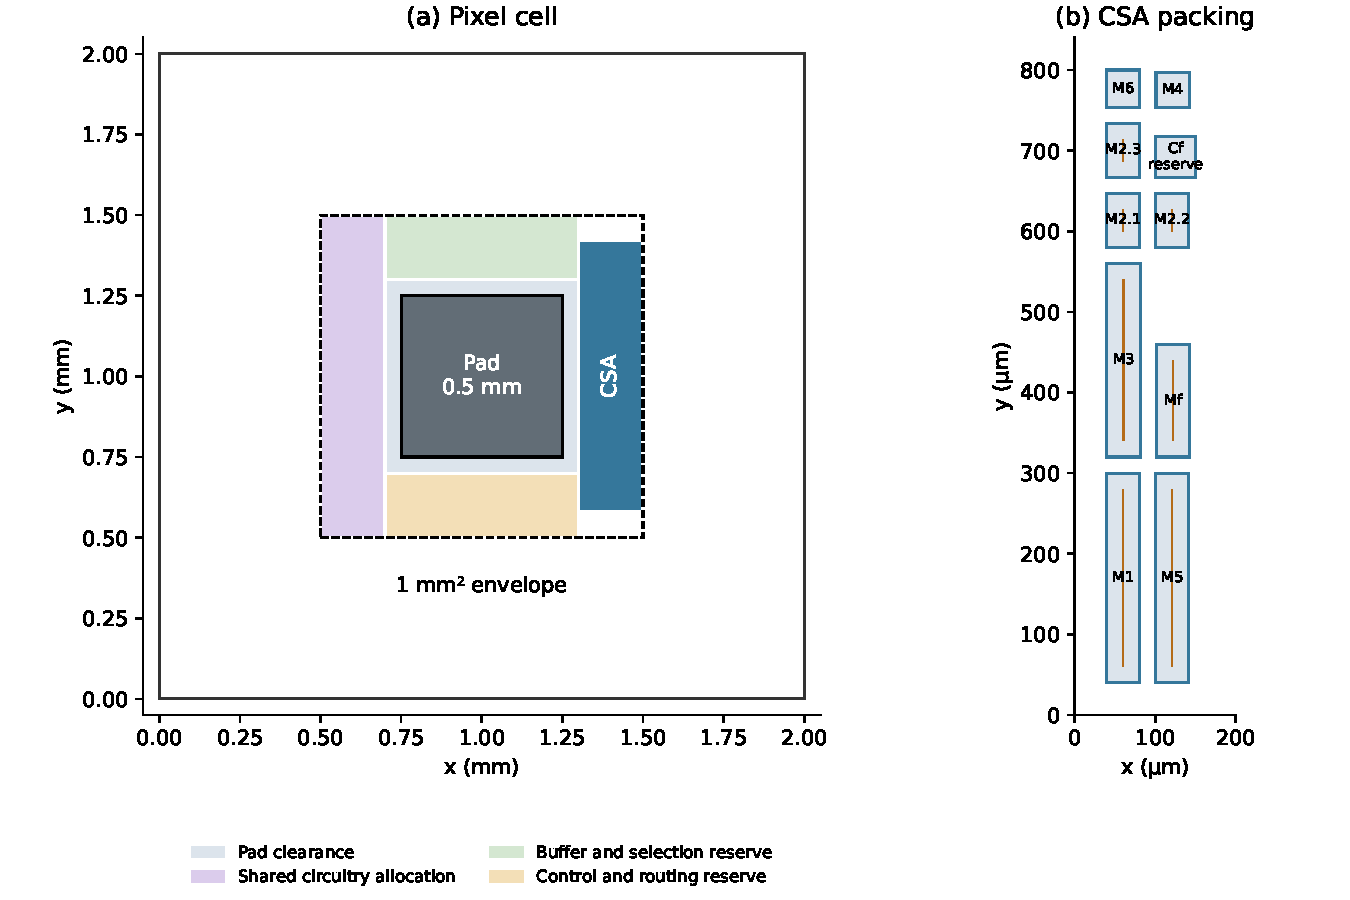
\includegraphics[width=\linewidth]{generated/pixel_area.pdf}
 \caption{Pixel area allocation. Left: the pad, CSA and reserves for readout,
 control and shared circuitry inside a \SI{\PixelBudgetArea}{\milli\metre\squared}
 envelope, shown within the full pixel cell. The shared circuitry block
 represents its area allocation per pixel. Right: packing of the transistor
 channels and their surrounding space, together with a reserve for the
 feedback capacitor.}
 \label{fig:pixel_area}
\end{figure}

\begin{table}[!htbp]
 \centering
 \begin{tabular}{lr}
\toprule
Block & Area (mm$^2$) \\
\midrule
Pad and clearance & 0.36 \\
CSA and feedback & 0.17 \\
Buffer and selection reserve & 0.12 \\
Control and routing reserve & 0.12 \\
Shared circuitry allocation & 0.20 \\
\midrule
Total & 0.97 \\
\bottomrule
\end{tabular}

 \caption{Pixel area budget for the arrangement in Fig.~\ref{fig:pixel_area}.}
 \label{tab:pixel_area}
\end{table}

\clearpage
\appendix
\section{Analytical single-ion response}
\label{app:single_ion}

\subsection{Weighting potential of a square pad}

The pad occupies $-a<x<a$, $-a<y<a$ in the plane $z=0$. Its weighting potential is one, and the remainder of the plane is held at zero. The upper half-space has uniform permittivity and no free charge in the weighting problem. The potential tends to zero at infinity. Thus $\nabla^2\phi_w=0$ for $z>0$, with a prescribed potential on the boundary.

Figure~\ref{fig:weighting_boundary} illustrates these boundary conditions:
\begin{equation}
 \begin{gathered}
 \phi_w(x,y,0)=
 \begin{cases}
  1, & |x|<a,\ |y|<a \quad \text{(pad)},\\
  0, & \text{elsewhere on the plane},
 \end{cases}\\
 \phi_w(\mathbf r)\longrightarrow0
 \quad\text{as }|\mathbf r|\longrightarrow\infty.
 \end{gathered}
 \label{eq:weighting_boundary}
\end{equation}
The values one and zero define the dimensionless weighting potential for this
pad. The operating voltages determine the physical field that drives the ions.

The half-space Poisson kernel gives~\cite{salazar2021}
\begin{equation}
 \begin{aligned}
 \phi_w(x,y,z)={}&\frac{1}{2\pi}\int_{-a}^{a}\int_{-a}^{a}\\
 &\frac{z\,\dd x'\,\dd y'}{[(x-x')^2+(y-y')^2+z^2]^{3/2}}.
 \end{aligned}
 \label{eq:app_poisson}
\end{equation}
The integral is the solid angle subtended by the pad, divided by $2\pi$. On the central axis, integration over the square yields
\begin{equation}
 \phi_w(z)=\frac{2}{\pi}\tan^{-1}
 \left[\frac{a^2}{z\sqrt{z^2+2a^2}}\right],\qquad z>0.
 \label{eq:app_square_phi}
\end{equation}
It approaches one at the pad and zero far from it. Differentiation gives the field in Eq.~\eqref{eq:single_weight}. At large distance,
\begin{equation}
 \phi_w(z)\simeq\frac{2a^2}{\pi z^2},\qquad
 W(z)\simeq\frac{4a^2}{\pi z^3}.
\end{equation}
The weighting field has units of inverse length because $\phi_w$ is dimensionless.

This boundary condition represents a metal pad surrounded by grounded metal. An exposed dielectric surface between pads would require a different solution. The actual IFG also modifies the weighting potential. The present expression is used as an analytical reference, with fixed electrode potentials and negligible perturbation of the physical field by the ion charge. Resistive materials can require time-dependent weighting fields~\cite{riegler2016,riegler2019}.

\subsection{Trajectory, charge and duration}
\label{app:single_duration}

The bulk operating point gives the mobility
\begin{equation}
 \mu=\frac{v_d}{E_{\rm bulk}}
 =\Mobility\times10^{-6}\ \mathrm{m^2/(V\,s)}.
\end{equation}
We use the same mobility in the nominal uniform gap field, giving $v=\mu E_g$. Diffusion during the final approach is omitted from the single-ion reference trajectory. The ion moves from $z=g$ to zero at this constant speed. Its induced current is Eq.~\eqref{eq:single_current}, and direct integration gives
\begin{equation}
 \int_{-g/v}^{0}i_1(t)\dd t
 =e\int_0^g W(z)\dd z
 =e[1-\phi_w(g)].
\end{equation}
For the example in Section~\ref{sec:single_ion}, $\phi_w(g)=\GapPotential$. The finite-path signal is not rescaled to $e$. Extending this trajectory to infinite distance gives $\int i_1\dd t=e$, but does not model passage through the IFG.

Inverting Eq.~\eqref{eq:app_square_phi} gives
\begin{equation}
 z(\phi)=a\sqrt{\frac{1}{\sin(\pi\phi/2)}-1}.
 \label{eq:app_inverse_phi}
\end{equation}
For the full reference trajectory, the interval immediately preceding collection that contains a fraction $F$ of the charge has duration
\begin{equation}
 T_F=\frac{z(1-F)}{v}.
\end{equation}
For a finite starting height $g$, the corresponding duration is
\begin{equation}
 T_{F,g}=\frac{z\!\left(1-F[1-\phi_w(g)]\right)}{v}.
\end{equation}
These definitions refer to integrated charge, not to the time above a fraction of the peak current. The pulse amplitude scales as $ev/a$, and its characteristic duration as $a/v$. Their product preserves the full-path charge.

For comparison, a circular pad of radius $a$ in the same grounded plane has
\begin{equation}
 \begin{aligned}
 \phi_{w,\circ}(z)&=1-\frac{z}{\sqrt{z^2+a^2}},\\
 W_\circ(z)&=\frac{a^2}{(z^2+a^2)^{3/2}}.
 \end{aligned}
\end{equation}
Its central peak is $ev/a=\SI{\DiskPeakCurrent}{fA}$ for the same lateral diameter as the square side, compared with \SI{\PeakCurrent}{fA} for the square. Both results assume the same constant velocity and grounded surroundings. Their difference illustrates shape dependence; it does not quantify the uncertainty of the real IFG--pad structure.

\subsection{Integration and feedback discharge}

For an ideal CSA, the input node remains at its reference potential. Current balance through the parallel feedback elements gives
\begin{equation}
 C_f\frac{\dd V_1}{\dd t}+\frac{V_1}{R_f}=-i_1(t).
\end{equation}
Multiplication by $\exp(t/\tau_f)$ and integration from $t_g=-g/v$ gives Eq.~\eqref{eq:csa_solution}. In the absence of discharge,
\begin{equation}
 V_1(t)=-\frac{e}{C_f}[\phi_w(-vt)-\phi_w(g)],
 \qquad t_g\leq t\leq0.
\end{equation}
The voltage remains at $-Q_g/C_f$ after collection. With finite $\tau_f$, its value at collection can also be written as
\begin{equation}
 V_1(0)=-\frac{e}{C_f}\int_0^g W(z)
 \exp\left(-\frac{z}{v\tau_f}\right)\dd z.
 \label{eq:app_csa_quadrature}
\end{equation}
This form permits an independent numerical check of the time-domain calculation.

Integrating the CSA equation between two readout times $t_{n-1}$ and $t_n$ gives the exact charge relation
\begin{equation}
 Q_n=-C_f\left[V_n-V_{n-1}
 +\frac{1}{\tau_f}\int_{t_{n-1}}^{t_n}V(t)\dd t\right],
 \label{eq:app_bucket_charge}
\end{equation}
where $Q_n$ is the induced input charge in that interval and $V_n=V(t_n)$. Thus the difference between samples gives the charge when discharge is negligible. With finite discharge, the correction depends on the voltage between samples. Recovering it from discrete samples requires a model or approximation for that interval.

If the current is constant over an interval $\Delta t$, its charge and the sampled voltages satisfy
\begin{equation}
 \begin{aligned}
 Q_n={}&-C_f\frac{\Delta t/\tau_f}{1-\exp(-\Delta t/\tau_f)}\\
 &\quad\times\left[V_n-\exp(-\Delta t/\tau_f)V_{n-1}\right].
 \end{aligned}
 \label{eq:app_bucket_constant}
\end{equation}
The limit $\tau_f\to\infty$ is $Q_n=-C_f(V_n-V_{n-1})$. Equation~\eqref{eq:app_bucket_constant} assumes constant current within the interval; two endpoint samples do not otherwise determine an arbitrary arrival history.

\subsection{Numerical evaluation and checks}

The current is represented by charge increments rather than point samples. For a time bin $[t_j,t_{j+1}]$ during the approach,
\begin{equation}
 q_j=e[\phi_w(-vt_{j+1})-\phi_w(-vt_j)].
\end{equation}
These increments sum exactly to the finite-path charge. Taking the bin-average current $q_j/\delta t$ gives the recurrence
\begin{equation}
 V_{j+1}=\alpha V_j
 -\frac{q_j}{C_f}\frac{\tau_f}{\delta t}(1-\alpha),
 \qquad \alpha=\exp(-\delta t/\tau_f).
 \label{eq:app_recurrence}
\end{equation}
This is exact for a constant current in each numerical bin and converges to the continuous-current solution as $\delta t$ decreases. The numerical step is separate from the readout sampling interval.

The square-pad potential is checked against independent surface integration of Eq.~\eqref{eq:app_poisson}, and its derivative against Eq.~\eqref{eq:single_weight}. Charge integrals, boundary limits and scaling with pad size and velocity are also checked. The CSA response is compared with Eq.~\eqref{eq:app_csa_quadrature}, the ideal-integrator limit and the closed-form response to a constant current. These checks test the analytical model and its numerical implementation; they do not replace a field calculation for the collection geometry or a transistor-level circuit calculation.

\section{Circuit and frame measurement}
\label{app:spice_readout}

\subsection{Circuit parameters}

The calculation uses BSIM3 transistor models for 180 nm CMOS, evaluated with
LTspice 17.2.4. Figure~\ref{fig:spice_circuit} gives the connections and gate
biases. Table~\ref{tab:spice_devices} gives the dimensions, including the
multiplicity $m$ of parallel devices. The pad capacitance is an external
load; intrinsic device capacitances are supplied by the transistor models.

The gate voltages of M3 and M4 are quoted as
\SI{\SpiceMthreeGateV}{V} and \SI{\SpiceMfourGateV}{V}, respectively.
Repeating the calculation with these rounded values changes the gain by
\SpiceBiasRoundingGainPercent\% and the ENC by
\SpiceBiasRoundingEncPercent\%.

The transient voltage is measured relative to a matched zero-input run.
The physical current has the square-pad boundary conditions specified in
Appendix~\ref{app:single_ion}; its integral is preserved in the tabulated
SPICE source. The gain $g$ is evaluated with the uniform arrival current,
the averaging windows and the frame difference defined in the main text.

\subsection{Contributions from neighbouring frames}

For equal-sized ion packets, the voltage left by a packet in the preceding
frame contributes \SpicePreviousPercent\% of the selected-frame signal
after the discharge correction. A packet collected in the following frame
contributes \SpiceFollowingPercent\%. Its ions induce current before reaching
the pad, and the voltage averaging window extends across the frame boundary.
Both contributions are calculated with the same averaging and discharge
correction used to recover the charge.

\subsection{Averaging and noise covariance}
\label{app:spice_noise}

Let $C_{\overline V}(u)$ be the covariance of averaged voltage readings
separated by $u$. For stationary noise with one-sided output spectrum $S_V$,
\begin{equation}
 C_{\overline V}(u)=\int_{f_\ell}^{f_h}S_V(f)
 \left|\frac{\sin(\pi fT_a)}{\pi fT_a}\right|^2
 \cos(2\pi fu)\,\dd f.
 \label{eq:spice_covariance}
\end{equation}
The same averaging window is applied to the transient signal. Squaring
Eq.~\eqref{eq:spice_noise_difference} and taking the average gives
\begin{equation}
 \sigma_D^2=(1+\alpha^2)C_{\overline V}(0)
           -2\alpha C_{\overline V}(\Delta t).
 \label{eq:spice_covariance_difference}
\end{equation}
Substituting Eq.~\eqref{eq:spice_covariance} yields
Eq.~\eqref{eq:spice_noise_integral}, since
\begin{equation}
 |1-\alpha e^{-2\pi\mathrm{i}f\Delta t}|^2
 =1+\alpha^2-2\alpha\cos(2\pi f\Delta t).
\end{equation}

The corrected difference retains a response $1-\alpha$ at zero frequency.
The lower integration limit $f_\ell$ therefore remains part of the noise
specification. The calculation uses the continuous average of the output
waveform and the circuit noise at its DC operating point.
ADC noise and quantisation must be included when a digitisation scheme is chosen.

The noise integral is checked by increasing the spectral sampling density
and the quadrature order. The signal is checked by reducing the transient
time step. Direct simulations of the adjacent integer ion counts bracket
the S/N threshold quoted in the main text.

Figure~\ref{fig:spice_averaging} shows how the averaging time affects the ENC.
Increasing the average from \SI{180}{\micro\second} to
\SI{350}{\micro\second} reduces the ENC from \SpiceScanFirstEnc\ to
\SpiceScanLastEnc\ electrons RMS. The signal per ion is recalculated for
each averaging time.

\begin{figure}[!htbp]
 \centering
 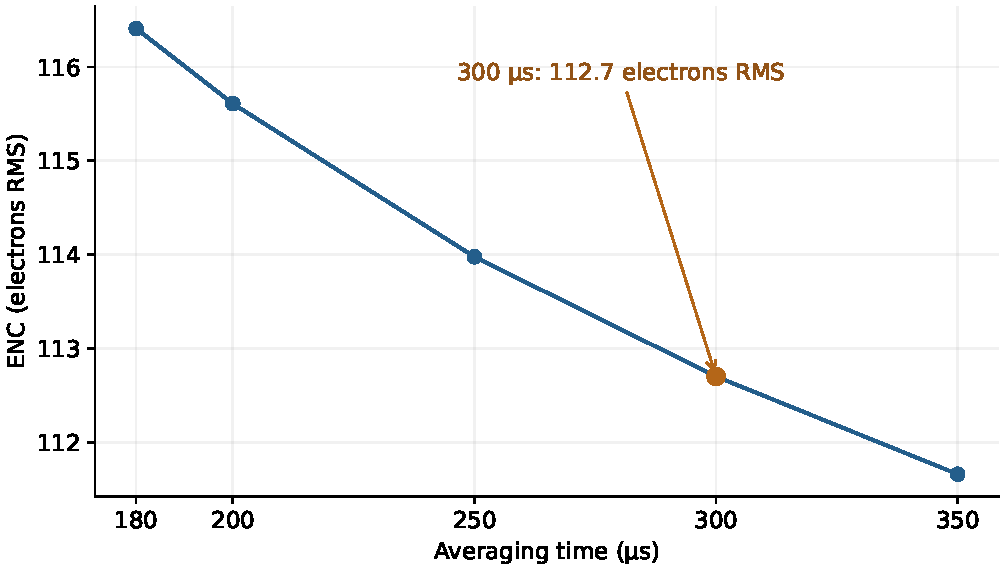
\includegraphics[width=0.88\linewidth]{spice_averaging.pdf}
 \caption{ENC versus averaging time for uniform ion arrivals over
 \SI{\SpiceFrameMs}{ms}, with an external pad capacitance of
 \SI{\SpicePadPf}{pF}. The highlighted point is the
 \SI{\SpiceAverageUs}{\micro\second} average used in this study.}
 \label{fig:spice_averaging}
\end{figure}

\section{Pixel area estimate}
\label{app:pixel_area}

The pad is centred in the pixel cell, with a clearance of
\SI{\PixelClearanceUm}{\micro\metre} on each side. The electronics are placed
outside this region. Each transistor channel is represented by a rectangle
with the dimensions in Table~\ref{tab:spice_devices}; the three parallel
instances of M2 are included separately. A margin of
\SI{\PixelDeviceMarginUm}{\micro\metre} is added on each side of each channel
to allow space for contacts, diffusion, wells and connections. These margins
are geometric allowances for the area estimate.

The rectangles are arranged in rows in a strip
\SI{\PixelCsaWidthUm}{\micro\metre} wide, with
\SI{\PixelRowGapUm}{\micro\metre} between neighbouring rectangles and
\SI{\PixelOuterMarginUm}{\micro\metre} at the outer boundary. A separate
rectangle reserves space for the feedback capacitor and its connections.
The resulting CSA block is \SI{\PixelCsaHeightUm}{\micro\metre} high.
The packing calculation checks that the rectangles do not overlap and
remain inside the allocated strip. Together with the readout, routing and
shared circuitry reserves in Table~\ref{tab:pixel_area}, this gives the
approximately \SI{\PixelBudgetArea}{\milli\metre\squared} budget.
This is a geometric estimate; a routed layout and parasitic extraction are
needed to determine the final circuit area and its effect on the noise.

\section{Comparison with Topmetal-S}
\label{app:topmetal}

Topmetal-S and NAUSICA use exposed metal electrodes connected to CSAs to
measure charge without gas amplification. A focusing electrode guides the
ions onto the collecting pads. Topmetal-S was developed to measure both
energy and track topology in a high-pressure ion TPC~\cite{mei2020topmetalcmosdirectcharge}.
In ITACA, electroluminescence provides the energy measurement, allowing
NAUSICA to choose its pitch and readout for ion-track imaging.

The Topmetal-S collecting electrode is a hexagon of \SI{1}{mm} diameter,
implemented in a 130 nm CMOS process~\cite{Liang2024TopmetalS}. The
N$\nu$DEx readout model places these electrodes at \SI{10}{mm}
pitch~\cite{Liang2026NvDExSimulation}. NAUSICA uses \SI{0.5}{mm} square
pads at \SI{2}{mm} pitch, close to the diffusion scale in ITACA. This
finer pitch samples the track with more pixels. The smaller pad reduces
the capacitive load, while the focusing field provides collection over
the pixel cell. The charge measured in each pixel must preserve the
track and its blob structure; the precise total-energy measurement is
provided by the electron signal.

\subsection{Noise measured with charge injection}

Topmetal-S reports an ENC of approximately $115\,e^-$ after a digital
trapezoidal filter~\cite{Yang2024TopmetalCSA}. Repeated injections of a
fixed charge produce a distribution of filtered pulse amplitudes. For
an injected charge of $N_{\rm inj}$ elementary charges, the ENC is
\begin{equation}
 \mathrm{ENC}=N_{\rm inj}\frac{\sigma_A}{\langle A\rangle},
\end{equation}
where $\langle A\rangle$ and $\sigma_A$ are the mean and standard deviation
of that distribution. The quoted noise therefore includes the effect
of the filter.

We perform a corresponding injection calculation for the circuit in
Table~\ref{tab:spice_devices}, with an external capacitance of
\SI{\SpicePadPf}{pF}. A pulse carrying
$\SpiceInjectionCalibration\,e$ has a \SI{1}{\micro\second} plateau
and \SI{10}{ns} rise and fall times. We apply a trapezoidal filter with
\SI{300}{\micro\second} rise time and \SI{300}{\micro\second} flat top.
The filtered voltage per elementary charge calibrates the signal. Applying
the same filter to the SPICE noise spectrum, including thermal and flicker
noise over \SI{\SpiceLowHz}{Hz}--\SI{\SpiceHighMHz}{MHz}, gives an ENC of
$\SpiceInjectionEnc\,e^-$ RMS. The calculation uses the supply and
temperature in Table~\ref{tab:spice_parameters} and noise evaluated at
the DC operating point.

\begin{table*}[!htbp]
 \centering
 \begin{tabular}{lll}
 \toprule
 & Topmetal-S & NAUSICA \\
 \midrule
 CMOS process & 130 nm & 180 nm \\
 Collecting electrode & \SI{1}{mm} diameter, hexagonal & \SI{0.5}{mm} side, square \\
 Pitch & \SI{10}{mm} (N$\nu$DEx model) & \SI{2}{mm} \\
 Injection ENC & $\sim115\,e^-$, measured & $\SpiceInjectionEnc\,e^-$, simulated \\
 \bottomrule
 \end{tabular}
 \caption{Geometry and charge-injection noise comparison. Both ENC values
 include trapezoidal filtering. The NAUSICA filter settings are given above;
 the Topmetal-S report~\cite{Yang2024TopmetalCSA} does not specify its
 trapezoid rise and flat-top durations.}
 \label{tab:topmetal_comparison}
\end{table*}


% Appendix C will contain the IFG focusing and collection calculation.
% That numerical study remains pending.

% Bibliography style is selected by sn-mathphys-num in the class options.
\bibliography{references}
\end{document}
